\documentclass[a4paper,12pt,oneside]{jex}
%\documentclass[a4paper,12pt,oneside]{jlreq}

\renewcommand{\baselinestretch}{1.1}
\setlength{\textwidth}{16cm}
\setlength{\textheight}{24cm}
\setlength{\evensidemargin}{0cm}
\setlength{\oddsidemargin}{0cm}
\setlength{\topmargin}{-1.0cm}

\usepackage[dvipdfmx]{graphicx}
\usepackage[dvipdfmx]{xcolor}
\usepackage[cmex10]{amsmath}
\usepackage[deluxe]{otf}
\usepackage{booktabs}
\usepackage{ascmac}
\usepackage{amssymb}
\usepackage{caption}
\usepackage{colortbl}
\usepackage{float} 
\usepackage{textcomp}
\usepackage{hyperref}
\usepackage{multirow,multicol}
\usepackage{wrapfig}
\usepackage{listings,jvlisting} 
\usepackage{mediabb}


\captionsetup{format=hang}
% ページの端に1行だけ残る段落を作らない
\widowpenalty=10000
\clubpenalty=10000
% 段落の途中でページを分けない
\interlinepenalty=10000
\raggedbottom

\lstset{
  basicstyle={\ttfamily\small},
  identifierstyle={\small},
  commentstyle={\small\itshape\color{gray}},
  keywordstyle={\small\bfseries\color{blue}},
  stringstyle={\small\ttfamily\color{brown}},
  showstringspaces=false,
  frame={tb},
  breaklines=true,
  columns=[l]{fullflexible},
  numbers=left,
  numberstyle={\scriptsize},
  stepnumber=1,
  numbersep=1zw,
  lineskip=-0.5ex
}

\pagestyle{headings}

%% ===== 表紙情報 =====
\title{
  \vspace{20mm}
  {\large アイディアソン レポート1}\\[8pt]
  {\LARGE 学校のAEDの利用可否の判断に向けた\\年間行事予定表からの休業日の取得}\\[8pt]
  {\large ― 浦安市の市立小中学校26校での検証 ―}\\[4pt]
}
\author{
  学生番号: 26G1087 \\
  氏名: 鄭家麒 \\[4pt]
}
\西暦
\date{提出日: \today}


\begin{document}

\thispagestyle{empty}
\setcounter{tocdepth}{3}

\pagenumbering{roman}
\pagenumbering{arabic}

\maketitle
%% ===== 概要 =====
\section*{概要}
千葉県では，救急車が5分未満で現場に到着した救急出場は1.7\%にとどまり，近くの人がAEDを使えるかどうかが救命を左右する．
しかし，学校のAEDの記録は「開校時のみ」などとするだけで，休業日の日付が書かれていない．
例えば浦安市では，AEDの記録288件のうち52件が市立小中学校のもので，すべて「開校時のみ」とだけ書かれている．
各校の休業日や行事の後の休校の日は，各校のWebサイトにある年間の予定表にしか載っていない．
浦安市の26校で調べると，トップページの「年間行事予定」などのリンクをたどるだけでは，表のある18校のうち5校の表を見落とした．
また，PDFから文字だけを取り出して近くの日付を拾う方法では，夏休みの期間を正しく求められたのは18校中1校，休校の日は57件中0件であった．
そこで本レポートでは，予定表の探し方を手順とキーワードで固定したツールと，表の中の文字の位置から各欄の日付を求める方法を提案した．
ツールは表のある学校をすべて見つけ，位置を使う方法では夏休みの期間を18校すべてで，休校の日を57件すべてで正しく求められた．
これにより，浦安市の学校のAEDの記録52件のうち38件で，休業日を日付で確かめられるようになった．

% 本文はここから
\section{はじめに}
\label{sec:introduction}

\subsection{背景}
\label{subsec:background}

心停止の人を救うには，AEDによる電気ショックをできるだけ早く行う必要がある．
千葉県の計画によると，市民がAEDを使用した傷病者の1か月後の生存率は53.8\%であった\cite{chiba_plan}．
一方，千葉県で救急車が5分未満で現場に到着した救急出場は1.7\%にとどまる\cite{chiba_r7}．
そのため，救急車が着く前に，近くの人がAEDを使えるかどうかが救命を左右する．

ただし，近くにAEDがあっても，その時に使えなければ役に立たない．
デンマークの研究では，心停止の近くにあったAEDがその時に使えた場合は，使えなかった場合に比べて，居合わせた人による電気ショックの割合が13.8\%対4.8\%，30日後の生存率が28.8\%対16.4\%であった\cite{karlsson}．
同じ研究で，学校・教育施設のAEDは，使えない時間があるために，近くで起きた心停止の66.7\%で使えなかった\cite{karlsson}．
AEDの適正配置に関するガイドラインも，AEDを可能な限り24時間使えるようにし，使用に制限がある場合はいつ使えるかを知らせることが望ましいとしている\cite{guide}．
つまり，AEDがいつ使えるかを前もって分かるようにすることが，救命につながる．

千葉県でも，使える日時が予定に左右されるAEDのうち，最も多いのは学校である．
千葉県オープンデータサイトのAEDデータ\cite{chiba_od}で，使える日時が施設の予定などで変わる記録617件を，「開校」「長期休業」などのキーワードで原因ごとに一つずつ分類すると，学校・園の年間の予定によるものが271件と最も多かった．

\subsection{問題点}
\label{subsec:problem}

しかし，学校のAEDの記録には，いつ使えるかが日付で書かれていない．
千葉県のAEDデータは，学校の予定を「開校時のみ」「長期休暇」など21通りの書き方で示すだけである\cite{chiba_od}．
例えば浦安市のAEDデータでは，288件の記録のうち52件（18.1\%）が市立小中学校26校のAEDであり，その52件はすべて「開校時のみ」とだけ書かれている\cite{urayasu_aed}．
この条件をある日に当てはめるには，その日が学校の休業日かどうかを知る必要があるが，休業日の日付はAEDのデータにも，市の「AED設置場所一覧」にも書かれていない\cite{urayasu_city}．

その結果，AEDを探す人は，ある日に学校のAEDが使えるかを判断できない．
休業日に学校へ向かえば，使えないAEDのために時間を失い，逆に開校日でも学校のAEDを候補から外せば，近くにある使えるAEDを見逃すおそれがある．
背景で述べたように，その時に使えるAEDがあるかどうかで，居合わせた人による電気ショックの割合や生存率は大きく変わる．
したがって，休業日が日付で分からないことは，学校のAEDによる救命の機会を減らしている．

そこで本レポートでは，学校のAEDの記録にある「開校時のみ」などの条件を，日付に当てはめられないことを問題とする．
この条件を字どおりに読むと，休業日は使えない日にあたる．
休業日に職員がいれば実際には使えるかという点は，記録に書かれた条件とは別の問題であり，第\ref{subsec:remain}節で述べる．

\subsection{技術的課題}
\label{subsec:issue}

休業日の日付を得る方法には，表\ref{tab:source}のようにいくつかある．
市や学校に問い合わせれば日付は分かるが，学校ごとに問い合わせる必要があり，予定が変わるたびに問い合わせ直さなければならない（第\ref{subsec:detail_problem}節）．
学校だよりにも予定は載るが，月ごとに出るため，1年分の休業日は一度には分からない．
これに対して，各校のWebサイトにある年間の予定表は，一つの資料で1年分の休業日と休校の日が分かり，浦安市では26校中19校が公開していた．
そのため本レポートでは，年間の予定表を使う．

\begin{table}[htbp]
\centering
\caption{学校の休業日の日付を得る方法の比較}
\label{tab:source}
{\small\setlength{\tabcolsep}{3pt}
\begin{tabular}{p{42mm}p{30mm}p{80mm}}
\toprule
\raggedright 方法 & \raggedright 休業日の日付 & \raggedright 問題 \tabularnewline
\midrule
\raggedright AEDのデータ，市のAED設置場所一覧 & \raggedright 書かれていない & \raggedright 「開校時のみ」「×」とあるだけ \tabularnewline
\raggedright 市や学校への問い合わせ & \raggedright 分かる & \raggedright 学校ごとに，予定が変わるたびに問い合わせる必要がある \tabularnewline
\raggedright 学校だより & \raggedright 1か月分ずつ分かる & \raggedright 月ごとに出るため，1年分は一度に分からない \tabularnewline
\raggedright 年間の予定表 & \raggedright 1年分が分かる & \raggedright 学校ごとに置き場所が違い，日付が表の位置で示される \tabularnewline
\bottomrule
\end{tabular}}
\end{table}

予定表を判断に使うには，予定表を集め，表から日付を取り出す必要がある．
しかし，どちらも素朴な方法では失敗する（第\ref{subsec:detail_issue}節）．

予定表を集めるとき，学校のトップページにある「年間行事予定」などのリンクを探すだけでは，名前や置き場所の違う表を見落とす．
そのため，リンクの名前や置き場所が学校ごとに違っても，目的の表を特定することが一つ目の技術的課題である．

また，予定表のPDFから文字だけを取り出し，行事名の近くの日付を拾うだけでは，表の上の「7月」などの見出しと各欄の行事との対応が失われ，正しい日付が得られない．
そのため，表の構造で示された行事と日付の対応を復元することが二つ目の技術的課題である．

\subsection{目的}
\label{subsec:aim}

本レポートの目的は，学校のAEDの記録にある「開校時のみ」などの条件を日付に当てはめられるように，各校の休業日と休校の日を，公開されている年間の予定表から日付で取り出すことである．
第\ref{sec:problem}章で問題点と技術的課題を詳しく示し，第\ref{sec:proposal}章で改善案を述べ，第\ref{sec:verification}章で改善案を検証する．

\section{問題点}
\label{sec:problem}

\subsection{問題点の詳細}
\label{subsec:detail_problem}

浦安市の学校のAEDの記録を，さらに詳しく調べた．
千葉県オープンデータサイトにある浦安市のAEDデータでは，市立小学校17校と中学校9校の計26校に，校舎と体育館の2件ずつ，計52件の記録がある\cite{urayasu_aed}．
52件の利用可能曜日の欄はすべて「開校時のみ」であり，曜日も時刻も休業日も書かれていない．
浦安市の公式サイトにある「AED設置場所一覧」でも，これらの学校の「24時間使用」の欄が「×」とされているだけで，いつ使えるかは書かれていない\cite{urayasu_city}．

第\ref{subsec:issue}節で述べたとおり，市や学校に問い合わせれば「開校時」の意味などの決まりは分かるが，休業日の日付は学校ごとに違い，年度の途中でも変わる．
例えば，浦安市の予定表には「令和8年4月10日現在」「令和8年3月25日現在」のように時点が書かれたものがあり，東小学校の予定表を載せたページは2026年10月23日より後に削除された．
また，浦安市のWebサイトでは，各校の休業日をまとめた一覧は見つからなかった．
そのため，休業日の日付は，問い合わせではなく，各校が公開する予定表から繰り返し取り出せることが望ましい．

特に，行事の後の休校は学校ごとに日が違い，他校の日付では補えない．
文字を読み取れる18校の表では，運動会などの後の学校全体の休校（振替休業）が計34日あり，14通りの日付に分かれていた（図\ref{fig:kyuko}）．
同じ校種の他校のうち半数より多くが休む日を，その学校の休校として補っても，正しかったのは34日のうち13日だけであった．
したがって，各校の予定表を一つずつ集めて読み取る必要がある．

\begin{figure}[htbp]
\centering
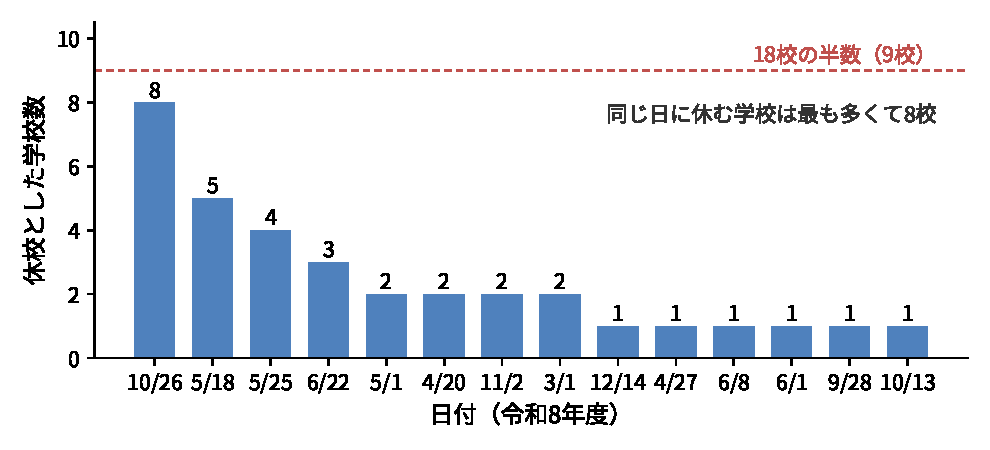
\includegraphics[width=140mm]{fig_kyuko.pdf}
\caption{浦安市の18校で，行事の後の休校とされた日付と，その日に休校とした学校の数．同じ日に休む学校は最も多くて8校で，半数（9校）に達する日はない．}
\label{fig:kyuko}
\end{figure}

\subsection{技術的課題の詳細}
\label{subsec:detail_issue}

\paragraph{予定表の有無}
浦安市の26校のWebサイトを調べると（2026年10月23日閲覧），令和8年度の年間の予定表があったのは19校で，7校にはなかった（表\ref{tab:urayasu}）．
調べ方は，市教育委員会の「学校一覧」\cite{urayasu_list}から各校のホームページに入り，「年間行事予定」などのリンクをたどる方法である．
7校のうち明海小学校には予定の表があったが，年度も日付も書かれておらず今年度のものか確かめられなかったため，「資料なし」とした．

\begin{table}[htbp]
\centering
\caption{浦安市の市立26校のWebサイトに載っていた令和8年度の予定}
\label{tab:urayasu}
\begin{tabular}{lr}
\toprule
載っていた予定 & 校数 \\
\midrule
年間の予定表（PDF） & 19 \\
月ごとの学校だよりだけ & 4 \\
月だけが書かれた表だけ（日付なし） & 1 \\
今年度の資料なし & 2 \\
\midrule
計 & 26 \\
\bottomrule
\end{tabular}
\end{table}

\paragraph{素朴な方法で予定表を集めた場合の失敗}
各校のトップページで，名前に「年間行事予定」「行事予定」を含むリンクだけをたどる方法を，2026年10月31日に試した．
その日に表を見つけられた18校のうち，この方法で見つかったのは13校であった．

見落とした5校のうち，美浜北小学校と日の出中学校ではトップページに該当する名前のリンクがなく，美浜北小学校の表は「令和8年度年間計画」という名前であった．
高洲小学校と明海南小学校では，表がトップページから2回以上リンクをたどった先のページに置かれていた．
明海中学校の表は，「保護者・地域の方へ」のページでPTAの資料の間に置かれていた．

筆者が手作業で探した場合も，2026年10月23日に19校のうち2校の表を見落とした．
1校はホームページの新着一覧にだけリンクがあった日の出小学校であり，もう1校は上の明海中学校である．
このほかにも，浦安中学校ではページ上部のメニューの「学校からのお知らせ」が過去の年度のページにつながっていたり，添付ファイルの欄が初めは閉じていてPDFが見えなかったりした．

\paragraph{文字だけで日付を拾った場合の失敗}
予定表の多くは，4月から3月までの12か月が横に並び，1日から31日までが縦に並ぶ表である．
日の出南小学校の表から文字を順に取り出すと，「1」「水」「学年始め休業」「金」「個人面談（希望制）」…「月」「短縮5時間下校14：10」「水」「土」「火」「始業式下校11：30」のように並ぶ．
これは4月1日から9月1日までの「1日」の行の文字が，月をまたいで横に続いたものであり，「始業式」が9月1日のことだとは，取り出した文字からは分からない．
「7月」「8月」などの月は表のいちばん上の見出しにしか書かれておらず，各欄の文字の近くには出てこないためである．

この方法で，夏休みの期間と行事の後の休校の日を求めた結果を表\ref{tab:moji}に示す．
夏休みの期間は，「終業式」「始業式」「夏季休業」の近くにある日付から求めた．
18校のうち13校では日付を一つも拾えず，4校では誤った期間になり，正しく求められたのは各欄に「7月17日」のように日付が書かれた1校だけであった．
誤った4校のうち3校は「夏季休業（～8/31）」の「8/31」を始まりの日とも取り違え，1校は近くにあった別の行事の「～7/28」を拾った．

休校の日は，「振替休業」「臨時休業」「代休」と書かれた欄57件で，近くの日付を拾った．
日付を拾えたのは12件だけで，そのすべてが誤りであった．
例えば「振替休業(5/16分)」からは，休校の日ではなく，もとの行事の日である5月16日を拾った．
また，各欄に日付が書かれた表でも，隣の月の欄の日付を拾った．

夏休みの示し方も，「夏季休業」と書かずに8月の欄を色で塗るだけの学校や，8月の列そのものがない学校など，8通りに分かれていた．

\begin{table}[htbp]
\centering
\caption{文字だけを取り出して近くの日付を拾う方法の結果（浦安市の18校）}
\label{tab:moji}
\begin{tabular}{lrrr}
\toprule
対象 & 件数 & 日付を拾えない & 正しい \\
\midrule
夏休みの期間 & 18 & 13 & 1 \\
行事の後の休校の日 & 57 & 45 & 0 \\
\bottomrule
\end{tabular}
\end{table}

以上をまとめると，二つのタスクを素朴な方法で行うと表\ref{tab:naive}のように失敗し，それぞれ第\ref{subsec:issue}節の技術的課題が生じる．

\begin{table}[htbp]
\centering
\caption{素朴な方法で生じる失敗と，解決すべき技術的課題}
\label{tab:naive}
{\small\setlength{\tabcolsep}{3pt}
\begin{tabular}{p{17mm}p{38mm}p{40mm}p{44mm}}
\toprule
\raggedright タスク & \raggedright 素朴な方法 & \raggedright 生じる失敗 & \raggedright 解決すべき技術的課題 \tabularnewline
\midrule
\raggedright 予定表を集める & \raggedright トップページの「年間行事予定」などのリンクを探す & \raggedright 名前や置き場所の違う表を見落とす（18校中5校） & \raggedright リンクの名前や置き場所が違っても，目的の表を特定する \tabularnewline
\raggedright 日付を取り出す & \raggedright PDFの文字を取り出し，行事名の近くの日付を拾う & \raggedright 月の見出しと欄の対応が失われ，日付を拾えないか誤る（休校57件中0件） & \raggedright 表の構造で示された行事と日付の対応を復元する \tabularnewline
\bottomrule
\end{tabular}}
\end{table}

\section{改善案}
\label{sec:proposal}

\subsection{予定表を集めるツール}
\label{subsec:collect}

一つ目の課題に対して，市教育委員会の学校一覧を入口に，各校のホームページとそこから1回のリンク先で，「年間」「行事」「予定」「だより」「お知らせ」などを含むリンクを自動でたどり，題名に「令和8年度」がある表を集めるツールを作る．
手順を図\ref{fig:steps}に示す．

\begin{figure}[htbp]
\centering
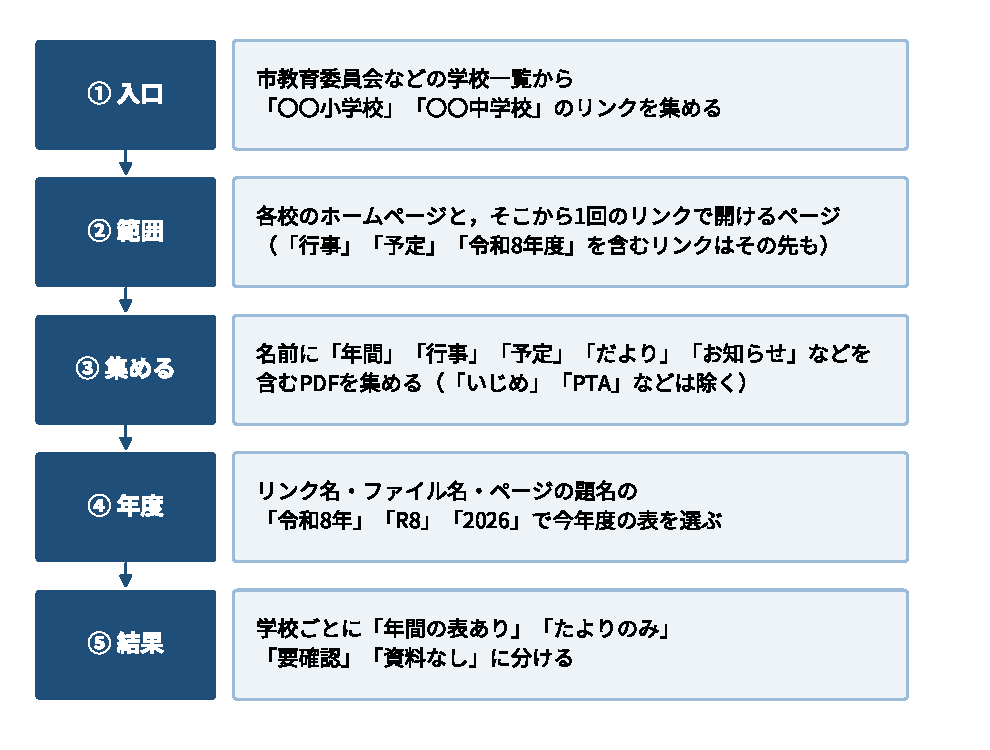
\includegraphics[width=130mm]{fig_steps.pdf}
\caption{予定表を集めるツールの手順．}
\label{fig:steps}
\end{figure}

素朴な方法との違いは，次の三つである．
第一に，トップページの特定の名前のリンクだけでなく，決めた範囲のページのリンクをすべて確かめる．
確かめる範囲は，各校のホームページと，そこから1回のリンクで開けるページまでとし，開いたページに「行事」「予定」「令和8年度」を含むリンクがあれば，その先も確かめる．
第二に，リンクの名前のキーワードを，浦安市の調査で実際に見られた名前から決め，「年間計画」のような別の名前も拾う．
第三に，WebページのHTMLを直接読むため，画面では閉じている添付ファイルの欄の中のPDFや，新着一覧の中のリンクも見落とさない．
入口を学校一覧にしたのは，検索エンジンで学校名を検索すると，同じ名前の他県の学校や過去の年度の資料が上位に出たためである．
題名に年度が書かれていない表は「要確認」として示し，人が開いて確かめる．
ツールはブラウザで動くJavaScriptで作り，手順とキーワードをプログラムに固定したため，同じ時点のサイトに対しては同じ結果が得られる．

\subsection{表の位置から日付を求める方法}
\label{subsec:position}

二つ目の課題に対して，表の中の文字の位置を使う．
PDFの文字にはページ上の位置が記録されているので，pdf.js\cite{pdfjs}で文字とその位置を取り出す．
そして，図\ref{fig:grid}のように，「7月」の列の「17」の行にある欄は7月17日というように，各欄の日付を求める．
年は年度から決め，4月から12月は2026年，1月から3月は2027年とする．

\begin{figure}[htbp]
\centering
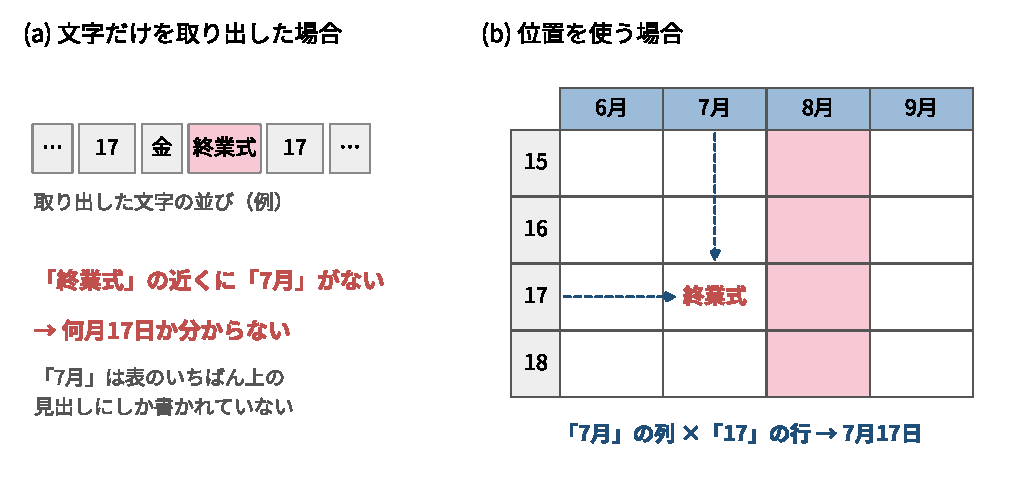
\includegraphics[width=150mm]{fig_grid.pdf}
\caption{文字だけを取り出した場合と，位置を使う場合の違い．}
\label{fig:grid}
\end{figure}

具体的には，表の上に「4月」「5月」などの見出しが並ぶ行を見つけ，各欄がどの見出しの下にあるかで月を決める．
日は，同じ行で欄の左にある日の数字から決める．
同じ行に曜日が書かれていれば，求めた日付の曜日と合うかを確かめる．
各欄の日付が分かれば，「振替休業」などと書かれた欄の日付がそのまま休校の日になる．
夏休みの期間は，始まりを「夏季休業」と書かれた欄の日付とし，なければ7月の終業式の翌日とする．
終わりは「～8/31」のような括弧の中の日付，「夏季休業終了」と書かれた欄の日付，2学期の始業式の前日の順で決める．
欄の色は学校ごとに塗り方が違い，土日と同じ色で塗られているため，期間を決めるのではなく，決めた期間を確かめるために使う．

\section{検証}
\label{sec:verification}

\subsection{検証の方法}
\label{subsec:method}

検証は，技術的課題が解決できたかと，問題点が改善されたかの二段階に分けて行った．
技術的課題の検証では，浦安市の26校で，目的の表を特定できるか（第\ref{subsec:v_collect}節）と，表の欄の日付を正しく求められるか（第\ref{subsec:v_date}節）を，素朴な方法と比べた．
「表がある学校」は，筆者の手作業とツールの結果を合わせ，すべての表を開いて確かめて決めた．
日付の正解は，筆者が表を目で見て決めた．
取り出せなかった休校がないかも，筆者が18校の表を目で見て確かめた．
問題点の検証では，取り出した情報によって，休業日を日付で確かめられるAEDの記録がどれだけ増えるかを数えた（第\ref{subsec:v_social}節）．

\subsection{技術的課題の検証：目的の表を特定する}
\label{subsec:v_collect}

結果を表\ref{tab:verify}に示す．
2026年10月31日には，素朴な方法は表のある18校のうち13校しか見つけられなかったが，ツールは18校すべての表を見つけた．
2026年10月23日には，手作業では19校のうち17校の表しか見つけられなかったが，ツールは19校すべての表を見つけた．
両日で表がある学校の数が違うのは，東小学校の表を載せたページが削除されたためである．

\begin{table}[htbp]
\centering
\caption{浦安市の26校で予定表を集めた結果}
\label{tab:verify}
\begin{tabular}{llrr}
\toprule
調べた日 & 方法 & 表がある学校 & 見つけた \\
\midrule
2026年10月31日 & 素朴な方法 & 18 & 13 \\
2026年10月31日 & ツール & 18 & 18 \\
2026年10月23日 & 手作業（筆者） & 19 & 17 \\
2026年10月23日 & ツール & 19 & 19 \\
\bottomrule
\end{tabular}
\end{table}

\subsection{技術的課題の検証：表の欄の日付を求める}
\label{subsec:v_date}

文字を読み取れる18校の表で，夏休みの期間と，「振替休業」「臨時休業」「代休」と書かれた欄57件の日付を求めた．
東小学校の表は，ページが削除された後もPDFのファイルが残っていたため，同じファイルを使った．
結果を表\ref{tab:date}に示す．
位置を使う方法では，夏休みの期間を18校すべてで，休校の日を57件すべてで正しく求められた．
表には，ほかに取り出せなかった休校はなかった．
57件のうち38件は学校全体の休校であり，19件は「6年振替休業」「けやき振替休業」のように学年や学級だけの休校であった．

\begin{table}[htbp]
\centering
\caption{表の欄の日付を正しく求められた数（浦安市の18校）}
\label{tab:date}
\begin{tabular}{lrrr}
\toprule
対象 & 件数 & 文字だけ & 位置を使う \\
\midrule
夏休みの期間 & 18 & 1 & 18 \\
行事の後の休校の日 & 57 & 0 & 57 \\
\bottomrule
\end{tabular}
\end{table}

求めた日付が正しいかは，表に書かれている祝日でも確かめた．
18校の表で「海の日」「山の日」などが書かれた欄の日付を，内閣府が公表する祝日\cite{holiday}と比べると，266件中264件が一致した．
一致しなかった2件は，学校の表の誤りであった．
1件は令和8年の山の日を8月10日としていたが，正しくは8月11日である．
もう1件は令和9年の春分の日を3月20日としていたが，正しくは3月21日である．

\subsection{問題点の検証：休業日が分かるAEDの記録}
\label{subsec:v_social}

改善案によって，浦安市の学校のAEDの記録52件のうち何件で休業日を日付で確かめられるようになるかを表\ref{tab:social}に示す．
現状では，52件のどれにも休業日の日付は書かれていない．
改善案により，年間の予定表を集められた19校の記録38件（73.1\%）で休業日を日付で確かめられるようになり，そのうち18校の36件（69.2\%）では夏休みの期間と休校の日を自動で求められた．

また，学校ごとに違う行事の後の休校34日について，他校の日付で補う方法では13日しか正しくなかったが，各校の表から求めると34日すべてが分かった．

\begin{table}[htbp]
\centering
\caption{浦安市の学校のAEDの記録52件のうち，休業日を日付で確かめられる記録}
\label{tab:social}
\begin{tabular}{lrr}
\toprule
& 件数 & 割合 \\
\midrule
現状（AEDデータのみ） & 0 & 0.0\% \\
改善案（年間の予定表を集められた学校の記録） & 38 & 73.1\% \\
\quad うち夏休みと休校の日を自動で求められた記録 & 36 & 69.2\% \\
\bottomrule
\end{tabular}
\end{table}

\subsection{本提案の限界}
\label{subsec:remain}

本提案では，26校のうち8校で休業日を自動で求められなかった．
その理由を表\ref{tab:remain}に示す．
表が画像だけのPDFの場合，文字とその位置を取り出せないため，表の位置から日付を求める方法は使えない．
また，年間の予定表が公開されていない学校や，表に年度や日付が書かれていない学校の休業日は，予定表を集める方法では分からない．

\begin{table}[htbp]
\centering
\caption{本提案で休業日を自動で求められなかった8校}
\label{tab:remain}
\begin{tabular}{ll}
\toprule
理由 & 学校 \\
\midrule
表が文字のない画像だけのPDF & 高洲小 \\
表に年度も日付も書かれていない & 明海小 \\
年間の表がなく，月ごとの学校だよりだけ & 4校 \\
日付の書かれた今年度の予定がない & 浦安小，入船中 \\
\bottomrule
\end{tabular}
\end{table}

次に，本提案は記録に書かれた「開校時のみ」という条件を日付に当てはめるものであり，この条件が実際の運用と合っているかは確かめていない．
休業日でも職員がいればAEDを使える場合があるかもしれないが，そのことは記録には書かれていない．
職員がいない日を表に示していた学校は，「閉庁日」と書いた1校と「日直を置かない日」と書いた3校の計4校だけであった．
そのため，ある日にAEDが実際に使えるかどうかは，市や学校に確かめる必要がある．

さらに，予定表は年度の途中で書き換えられたり，置き場所が変わったりする．
東小学校の表を載せたページが削除されたように，一度集めた結果がいつまでも正しいとは限らないため，定期的に集め直す必要がある．

\section{おわりに}
\label{sec:conclusion}

本レポートでは，学校のAEDがある日に使えるかを判断するために必要な休業日と休校の日を，公開されている予定表から取り出すため，予定表を集めるツールと，表の位置から日付を求める方法を提案した．
浦安市の26校では，ツールは素朴な方法や手作業で見落とした表も含めてすべての表を見つけた．
また，表の中の文字の位置を使うことで，夏休みの期間を18校すべてで，学校ごとに違う休校の日を57件すべてで正しく求められた．
これにより，浦安市の学校のAEDの記録52件のうち38件で，休業日を日付で確かめられるようになった．

一方で，画像だけの表や，予定が公開されていない学校の休業日は，本提案では分からない．
また，休業日に職員がいればAEDを使えるのかは，公開されている情報からは分からない．
今後は，他の市でもツールを試して手順とキーワードを確かめるとともに，学校の休業日と職員のいない日を，AEDの判断に使える形で公開してもらうことが必要である．


% 参考文献
% URLを任意の文字の後で改行できるようにする（長いURLが右端からはみ出さないように）
\makeatletter
\providecommand{\UrlBreaks}{}
\g@addto@macro{\UrlBreaks}{\do\a\do\b\do\c\do\d\do\e\do\f\do\g\do\h\do\i\do\j\do\k\do\l\do\m\do\n\do\o\do\p\do\q\do\r\do\s\do\t\do\u\do\v\do\w\do\x\do\y\do\z\do\A\do\B\do\C\do\D\do\E\do\F\do\G\do\H\do\I\do\J\do\K\do\L\do\M\do\N\do\O\do\P\do\Q\do\R\do\S\do\T\do\U\do\V\do\W\do\X\do\Y\do\Z\do\0\do\1\do\2\do\3\do\4\do\5\do\6\do\7\do\8\do\9\do\_\do\(\do\)}
\makeatother
\begin{thebibliography}{10}

\bibitem{chiba_plan}
千葉県.
\newblock {千葉県ＡＥＤ等普及促進計画}.
\newblock 千葉県公式Webサイト, 2021.
\newblock 最終アクセス日: 2026年10月18日.
\newblock URL:
  \url{https://www.pref.chiba.lg.jp/iryou/taiseiseibi/aed/documents/AEDkeikaku.pdf}.

\bibitem{chiba_r7}
千葉県.
\newblock {令和7年版消防防災年報 第3表
  救急隊覚知からの現場到着所要時間別出場件数}.
\newblock 千葉県オープンデータサイト, 2026.
\newblock 最終アクセス日: 2026年10月18日.
\newblock URL: \url{https://opendata.pref.chiba.lg.jp/resources/49853}.

\bibitem{karlsson}
Lena Karlsson, Carolina Malta Hansen, Mads Wissenberg, et al.
\newblock {Automated external defibrillator accessibility is crucial for bystander defibrillation and survival: A registry-based study}.
\newblock Resuscitation, Vol. 136, pp. 30--37, 2019.
\newblock 最終アクセス日: 2026年10月31日.
\newblock URL: \url{https://doi.org/10.1016/j.resuscitation.2019.01.014}.

\bibitem{guide}
一般財団法人日本救急医療財団.
\newblock {AEDの適正配置に関するガイドライン}.
\newblock 厚生労働省Webサイト, 2018.
\newblock 最終アクセス日: 2026年10月18日.
\newblock URL: \url{https://www.mhlw.go.jp/content/10800000/000748008.pdf}.

\bibitem{chiba_od}
千葉県.
\newblock {千葉県オープンデータサイト データセット一覧「AED」}.
\newblock 千葉県オープンデータサイト.
\newblock 最終アクセス日: 2026年10月16日.
\newblock URL: \url{https://opendata.pref.chiba.lg.jp/datasets?keyword=AED}.

\bibitem{urayasu_aed}
浦安市.
\newblock {【浦安市】AED設置箇所一覧（2026.3.23）}.
\newblock 千葉県オープンデータサイト, 2026.
\newblock 最終アクセス日: 2026年10月24日.
\newblock URL: \url{https://opendata.pref.chiba.lg.jp/resources/56482}.

\bibitem{urayasu_city}
浦安市.
\newblock {浦安市AED（自動体外式除細動器）設置場所一覧}.
\newblock 浦安市公式サイト, 2026.
\newblock 最終アクセス日: 2026年10月30日.
\newblock URL: \url{https://www.city.urayasu.lg.jp/todokede/anzen/kyukyu/1029669.html}.

\bibitem{urayasu_list}
浦安市教育委員会.
\newblock {学校一覧}.
\newblock 浦安市教育委員会Webサイト.
\newblock 最終アクセス日: 2026年10月23日.
\newblock URL: \url{https://www.city-urayasu.ed.jp/}.

\bibitem{pdfjs}
Mozilla.
\newblock {PDF.js}.
\newblock GitHub.
\newblock バージョン3.11.174を使用．最終アクセス日: 2026年10月23日.
\newblock URL: \url{https://github.com/mozilla/pdf.js}.

\bibitem{holiday}
内閣府.
\newblock {「国民の祝日」について}.
\newblock 内閣府Webサイト.
\newblock 令和8年及び令和9年の国民の祝日の一覧を使用．最終アクセス日: 2026年10月23日.
\newblock URL: \url{https://www8.cao.go.jp/chosei/shukujitsu/gaiyou.html}.

\end{thebibliography}

\end{document}
